\scanpage{57}
\mspage{56}

\uline{Proposition} a) Si $F$ \deleted{\unsure{est|était}} est une figure, alors les figures $F'$ telles que $F'\leq F$ s'identifient, par l'application $F'\mapsto\overline F'$, aux parties de $\overline F$ qui sont \uline{fermées} pour la relation d'ordre \inserted{$\leq$} de $M$.

b) Si $F$ et $G$ sont deux figures, $F\wedge G$ existe (inf pour $\leq$) \inserted{\uuline{figure intersection}} et \deleted{\unsure{des|les|on|en}} $\overline{F\cap G}=\overline F\cap\overline G$. Même pour une famille $(F_i)_{i\in I}$ quelc. \inserted{avec \uline{\uuline{$I\neq\phi$}}}.

% Two marginal callout strokes, reproduced beside the associated additions.
\figure{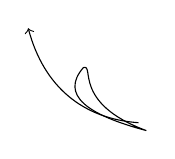
\begin{tikzpicture}[x=1cm,y=1cm]
\draw[->] (1.4,0) .. controls (.7,.05) and (.2,.45) .. (0,1.2);
\draw (1.5,-.1) .. controls (.55,.25) and (.85,.75) .. (.7,.7) .. controls (.4,.35) and (.75,.1) .. (1.5,-.1);
\end{tikzpicture}}
% margin note written sideways
\margin{\uline{Mais attention} il vaut mieux ne pas \unsure{le|les} noter $F\cap G$, car quand il y a une notion de support, ça ne correspond pas à l'intersection des supports, \unsure{sauf si} $F,G$ compatibles.}

[ \uline{Lieux} de $\mathcal F$ : ce sont les \deleted{\unsure{par|pas|pet}} figures qui sont \uline{minimales} dans $\mathcal F\setminus\{\phi_{\mathcal F}\}$. \deleted{\unsure{Un|Une},} \deleted{Un lieux est de \unsure{ce nom|nom}}  Tout lieu est irréductible. Donc les lieux sont aussi les éléments minimaux de $ M$ : ce sont les multistrates qui n'ont d'autres strates \unsure{qu'elle-même|qu'elles-même}. ] \deleted{Si $F$ est une \unsure{figure|figures}, les}

% slanted
\margin{Définition \unsure{car un lieu|courante} n'est \unsure{raisonnable|raisonn.ble} que dans certains cas \deleted{\unsure{(quand les|(quand la}} (p. ex. les \unsure{contrées|centrés} en boules'', ou contrées \unsure{par morceaux|premiers} $\ldots$) Car dans les cas types d'ordre quelconq., un \unsure{modèle|modélé} $\overline E$ \unsure{de str.|de structure} \unsure{semi-}\illegible{1} \inserted{\unsure{univers vides|univers vide|non-vide}\unsure{,|)}} \unsure{forme|formée|fermée} \deleted{\unsure{peut être une|peut être un}} \inserted{une} multistrate \unsure{minimale|minime}, \unsure{mais on ne l'appelle|mais on ne appelle|n'est} un ``lieu'' que si elle est \unsure{vide réel|vide réelle|vide} !}

\uline{Figures} \uline{disjointes} \unsure{,,|''} \uline{$F$} et \uline{$G$} : telles que a) $F$ et $G$ compatibles, i.e $F\cup G$ existe \deleted{et b)} ou encore $\{F,G\}$ majoré pour $\leq$ et b) $F\cap G=\phi_{\mathcal F}$ \deleted{\unsure{ou|et} Cela signifie \unsure{donc|que}} \inserted{(i.e. $\overline F\cap\unsure{\overline G|G}=\phi$)}.

% Long curved separator beside the lower margin and proposition.
\figure{\begin{tikzpicture}[x=1cm,y=1cm]\draw (.6,3) .. controls (.2,2.3) and (.05,1.3) .. (.15,.9) .. controls (.2,.3) and (.4,.05) .. (.65,0);\end{tikzpicture}}
% slanted
\margin{\unsure{Bloquer|bloque} \unsure{avec|mes} ``\unsure{complémentaires|composantes}''}

\deleted{Si $F$ et $G$ sont} \uline{Prop} Si $F$ et $G$ sont disjointes, alors pour $F'\leq F$, $G'\leq G$, $F'_{\unsure{a|\deleted{a}}}$ et $G'$ sont disjointes, et $F'\cup G'$ est une sous figure de $F\cup G$, l'application $(F'\unsure{;|,}G')\mapsto F'\cup G'$ est une bijection \deleted{de l'ens de $\unsure{\mathcal F|F}$}
